% ---------------------------------------------------------------------------
% paper_zh.tex -- 中文版（阅读与内部评审用，非投稿件）
%
% 用 xelatex 编译：xelatex paper_zh.tex （跑两遍以定位交叉引用）
% 依赖：fontspec + Noto Serif/Sans CJK SC 字体
%
% 这是 paper.tex 的完整译文，内容一一对应。数值、公式编号、参考文献编号
% 与英文版一致，便于对照。投稿以英文版为准。
% ---------------------------------------------------------------------------
\documentclass[10pt,twocolumn]{article}
\usepackage[margin=0.75in]{geometry}
\usepackage{fontspec}
\usepackage{amsmath,amssymb,amsthm,graphicx,bm}
\usepackage[colorlinks=true,linkcolor=blue,citecolor=blue,urlcolor=blue]{hyperref}
\usepackage{url}
\usepackage{titlesec}

\setmainfont{Noto Serif CJK SC}
\newfontfamily\headingfont{Noto Sans CJK SC}
\XeTeXlinebreaklocale "zh"
\XeTeXlinebreakskip = 0pt plus 1pt minus 0.1pt

\titleformat{\section}{\normalfont\headingfont\bfseries\filcenter}{\Roman{section}.}{0.5em}{}
\titleformat{\subsection}{\normalfont\headingfont\filcenter}{\Alph{subsection}.}{0.5em}{}
\setlength{\parskip}{2pt}
\linespread{1.06}

\newcommand{\tenB}{$^{10}$B}
\newcommand{\elevenB}{$^{11}$B}
\newcommand{\kzero}{k_{0}}
\newcommand{\Tr}{\mathcal{T}}
\newtheorem*{thm}{定理}

\begin{document}

\twocolumn[
\begin{center}
{\headingfont\bfseries\large
声子输运的超均匀同位素工程：\\
精确标度律与六方氮化硼中的隐形透明窗口\par}
\vspace{8pt}
{吴荣华\textsuperscript{1}，陈汝清\textsuperscript{2}\par}
\vspace{4pt}
{\small\textsuperscript{1}珠海九重天航空科技有限公司，中国珠海\quad wrh@gdtzn.com\\
\textsuperscript{2}GUT Geoservice Inc.，加拿大蒙特利尔\quad ruqing@hotmail.com\par}
\vspace{10pt}
\end{center}
\begin{minipage}{0.86\textwidth}
\small
\textbf{摘要}\quad
同位素替换是晶体中极少数严格的纯质量微扰之一：在玻恩--奥本海默近似下，原子间力常数在同位素交换下逐元素不变，因此同位素图案仅通过质量因子改变动力学矩阵。这使得同位素的\emph{空间排布}成为一个设计变量，独立于迄今同位素工程唯一关注的同位素方差 $g_2$。我们引入质量涨落结构因子 $S_\epsilon(\bm k)=g_2\,s(\bm k)$，将 Tamura 声子--同位素散射理论推广到空间关联的排布，并证明当小波数极限下 $s(k)\simeq(k/\kzero)^\alpha$ 时，$d$ 维中的弛豫率服从精确标度律 $\tau_{\rm iso}^{-1}\propto\omega^{\,d+1+\alpha}$，其角平均前因子有闭式解 $2/(\alpha+2)$。因此超均匀性指数对瑞利指数的贡献是一个可加的、与维度无关的修正，与维度基线正交。我们用具有高斯酉系综（GUE）间距统计的序列实现 Class~II 情形 $\alpha=1$——黎曼 zeta 函数的展开非平凡零点是其典范例子——将其映射到六方氮化硼的一维 \tenB/\elevenB\ 调制上，得到 $\tau_{\rm iso}^{-1}\propto\omega^5$ 以取代瑞利的 $\omega^4$。我们进一步在数值上发现，由有限高度零点构成的序列比 GUE 更刚性，给出 $\alpha=1.49\pm0.12$，且该指数与所用零点的高度无关：在跨越 $\bar\gamma=1.2\times10^{3}$ 到 $6.2\times10^{7}$ 的八个互不重叠窗口上，拟合趋势为 $-0.138\pm0.075$，与零一致，因此这一更深的压制无需任何调参即可获得。对于隐形（Class~I）排布，我们证明黄金规则散射率在 $\omega<vK/2$ 时\emph{恒等于}零，而非渐近趋零，其中 $K$ 为隐形波数。我们提出以配比匹配样品之间的差分透射 $\Delta\Tr(\omega)$ 作为观测量，它在一阶上抵消 Casimir 与非谐背景；在液氦温区确定了 $4$--$7$~THz 的可行观测窗口；并将由此导出的制备指标——$1.25$~nm 调制间距、$300\,\mu$m 长度——作为明确的设计目标提出，该指标超出当前生长能力。
\vspace{10pt}
\end{minipage}
]

\section{引言}
\label{sec:intro}

自金刚石与硅的最早工作以来，声子输运的同位素工程一直围绕单一标量组织，即质量方差
\begin{equation}
  g_2 = \sum_i f_i\left(1-\frac{m_i}{\bar m}\right)^{\!2},
  \label{eq:g2}
\end{equation}
其中 $f_i$ 为同位素 $i$ 的丰度。通过同位素提纯降低 $g_2$ 已在金刚石、硅、砷化硼中产出创纪录的热导率，最引人注目的是立方氮化硼：富集至任一硼同位素 $99\%$ 时室温热导率超过 $1600~\mathrm{W\,m^{-1}K^{-1}}$~[1]。在六方氮化硼中，同一策略将面内热导率提升至 $585~\mathrm{W\,m^{-1}K^{-1}}$~[2]，并显著延长双曲声子极化激元寿命~[3]。

以上工作全部把同位素分布视为\emph{随机}。支撑它们的 Tamura 与 Klemens 理论明确假定不同格点上的同位素占据互不关联~[4,5]；在该假定下质量涨落结构因子是白的，整个同位素问题因而坍缩为 $g_2$。

然而在\emph{生长}出的晶体中，这一假定没有物理上的必然性。原则上，逐层前驱体切换允许任意指定的序列。本文要问的是：当排布在固定 $g_2$ 下被当作设计变量时，能够获得什么。

描述此类排布的自然语言是超均匀性。当一个点图案的结构因子在无限波长极限下趋于零时称其为超均匀，此时长波长密度涨落被反常压制~[6,7]。Torquato 的分类按 $S(k)\sim|k|^\alpha$ 中的指数 $\alpha$ 组织超均匀体系：Class~I（$\alpha>1$，包含全部晶体与准晶）、Class~II（$\alpha=1$，数方差按对数增长）、Class~III（$0<\alpha<1$）。随机排布对应 $\alpha=0$。

长波声子恰恰对超均匀性所压制的那类涨落敏感。我们在下文确立：同位素散射指数以一种简单的可加方式受 $\alpha$ 控制。

为实现特定的 $\alpha$，我们需要一个小波数结构因子已知精确形式的序列。黎曼 zeta 函数的非平凡零点提供了典范例子。依据 Montgomery--Odlyzko 对应~[10,11]，展开后的零点具有与高斯酉系综（GUE）本征值相同的对关联统计，Dyson 的精确解给出闭式
\begin{equation}
  s_{\rm GUE}(k)=
  \begin{cases}
    k/2\pi, & k<2\pi,\\[2pt]
    1,      & k\ge 2\pi,
  \end{cases}
  \label{eq:sgue}
\end{equation}
（以单位平均间距为单元）。这精确地是 $\alpha=1$，无需拟合。

必须强调，零点在此纯粹作为一个数学上精确的 Class~II 序列生成器出现。下文所有预言仅通过 $\alpha$ 依赖于排布，任何 $\beta=2$ 的能级排斥点过程都能同样胜任。选择零点是因为其结构因子有闭式解，而非因为该序列本身具有任何被假定的意义。

\section{理论框架}
\label{sec:theory}

\subsection{质量微扰的精确性}

在玻恩--奥本海默近似下，原子核质量不进入电子哈密顿量。二阶力常数张量
\begin{equation}
  \Phi_{ij}^{\alpha\beta}
    = \frac{\partial^{2}E}{\partial u_i^\alpha\,\partial u_j^\beta}
  \label{eq:phi}
\end{equation}
因此在同位素替换下逐元素不变，仅动力学矩阵中的质量因子改变，
\begin{equation}
  D(\bm q)=M^{-1/2}\,\Phi(\bm q)\,M^{-1/2}.
  \label{eq:dynmat}
\end{equation}

由此产生两个后果。物理上，同位素图案在不形变势能面的前提下探测声子本征矢。计算上，$\Phi$ 只需在原胞上计算一次；此后任意排布均可通过置换对角矩阵 $M$ 零额外第一性原理成本地获得（见第~\ref{sec:methods}~节）。

记 $M_n=\bar M(1+\epsilon_n)$，$\epsilon_n\equiv\Delta M_n/\bar M$，则
\begin{equation}
  \delta D = -\,\omega^{2}\sum_n \epsilon_n\,|n\rangle\langle n|
             + \mathcal{O}(\epsilon^{2}).
  \label{eq:deltaD}
\end{equation}
对 \tenB/\elevenB\ 对有 $|\epsilon|\lesssim0.05$，故二阶贡献被压制 $\sim10^{-3}$；其作用在第~\ref{sec:stealthy}~节定量给出。

\subsection{广义 Tamura 公式}

Bloch 态之间的矩阵元为
\begin{equation}
  \langle\bm q'|\delta D|\bm q\rangle
    = -\frac{\omega^{2}}{N}\sum_n \epsilon_n\,
      e^{i(\bm q-\bm q')\cdot\bm R_n}.
  \label{eq:matelem}
\end{equation}
定义\textbf{质量涨落结构因子}
\begin{equation}
  S_\epsilon(\bm k)\equiv
    \frac{1}{N}\left|\sum_n \epsilon_n e^{i\bm k\cdot\bm R_n}\right|^{2}
    = g_2\,s(\bm k),
  \label{eq:Seps}
\end{equation}
其中 $s$ 在大 $k$ 极限归一至 $1$。费米黄金规则给出
\begin{equation}
  \frac{1}{\tau(\omega)}
    = \frac{\pi}{2}\,\omega^{2}D(\omega)
      \big\langle S_\epsilon(|\bm q-\bm q'|)\big\rangle_{\rm FS},
  \label{eq:tamura}
\end{equation}
$\langle\cdot\rangle_{\rm FS}$ 表示等频面上的平均。

式~\eqref{eq:tamura} 是本工作的中心关系。它相对标准 Tamura 结果的唯一推广是因子 $s(\bm k)$；令 $s\equiv1$ 即精确回到不关联理论。排布工程的全部内容都居于 $s$ 的小 $k$ 行为之中。与原始工作一样，它是虚晶背景上的一阶 Born 处理，其在强散射或光学支情形下的局限见文献~[12]；对本文所考虑的弱 \tenB/\elevenB\ 质量对比，这些修正可以忽略。

关于适用性的两点说明。其一，式~\eqref{eq:tamura} 是 $\epsilon$ 的一阶，描述单次散射过程；多次散射见第~\ref{sec:stealthy}~节。其二，在多子晶格情形下右端需乘以 Tamura 原始处理中的本征矢投影 $\sum_\kappa g_2(\kappa)|\bm e(\kappa|\bm q,j)|^{2}$。在 h-BN 中该因子严重不对称：天然氮（$99.64\%$ $^{14}$N）的氮子晶格贡献 $g_2\approx1.8\times10^{-5}$，比等摩尔硼子晶格低两个数量级，故硼投影占主导。全文保留标量形式，仅在给出数值时恢复该投影。

\subsection{排布的分类}

设
\begin{equation}
  s(k)\simeq(k/\kzero)^{\alpha},\qquad k<\kzero,
  \label{eq:alphadef}
\end{equation}
$\kzero$ 为 $s$ 饱和的交叉波数。随机合金给出 $\alpha=0$；Class~III 为 $0<\alpha<1$；Class~II（GUE、黎曼零点）为 $\alpha=1$，数方差 $\sigma^{2}(R)\sim R^{d-1}\ln R$；Class~I（周期、准周期、隐形）为 $\alpha>1$。随机矩阵谱、数论与超均匀点过程之间的联系见文献~[9]。对零点映射，式~\eqref{eq:sgue} 配以物理平均间距 $\ell$ 给出 $\kzero=2\pi/\ell$ 与精确的 $\alpha=1$。

\subsection{精确标度律}
\label{sec:scaling}

将式~\eqref{eq:alphadef} 代入式~\eqref{eq:tamura}。三维情形下等频面上的动量转移为 $k=2q\sin(\theta/2)$，作代换 $u=\sin(\theta/2)$ 后角平均有闭式解，
\begin{equation}
  \big\langle k^{\alpha}\big\rangle
    = (2q)^{\alpha}\!\!\int_0^{\pi}\!\!\sin^{\alpha}\!\tfrac{\theta}{2}
      \cdot\tfrac{1}{2}\sin\theta\,d\theta
    = (2q)^{\alpha}\,\frac{2}{\alpha+2}.
  \label{eq:angavg}
\end{equation}
结合德拜态密度 $D(\omega)\propto\omega^{2}$，
\begin{equation}
  \boxed{\;
  \frac{1}{\tau_{\rm 3D}(\omega)}
    = \frac{V_0\,g_2}{4\pi v^{3}}\,\omega^{4}\cdot\frac{2}{\alpha+2}
      \left(\frac{2\omega}{v\kzero}\right)^{\!\alpha}\;}
  \label{eq:master3d}
\end{equation}
适用于 $\omega<v\kzero/2$；在此之上 $s\to1$，回到瑞利形式。当 $\alpha=0$ 时前因子退化为 $1$，式~\eqref{eq:master3d} 精确成为 Klemens 结果，这在无可调参数的情况下固定了归一化。

在一般维度重复推导，取 $D(\omega)\propto\omega^{d-1}$，得到紧凑陈述
\begin{equation}
  \boxed{\;\frac{1}{\tau_{\rm iso}}\;\propto\;\omega^{\,d+1+\alpha}\;}
  \label{eq:master}
\end{equation}

\textbf{超均匀性对瑞利指数贡献一个可加的、与维度无关的修正 $+\alpha$。} 维度设定基线（体材料 $\omega^{4}$，单层 $\omega^{3}$，量子化准一维通道 $\omega^{2}$），排布提供修正；二者正交。式~\eqref{eq:master} 是本工作的主要解析结果。

需注意一点。式~\eqref{eq:master} 假定了德拜形式的 $D(\omega)$。在层状 h-BN 中，声学色散仅在层间交叉频率以下是三维的；在此之上态密度趋于二维形式，基线指数从 $4$ 向 $3$ 漂移。可加项 $+\alpha$ 不受影响，因为它完全源自 $s(k)$，但绝对指数必须从计算得到的 $D(\omega)$ 提取，而非假定。

取 $\alpha=1$、$\kzero=2\pi/\ell$，
\begin{equation}
  \frac{1}{\tau_{\rm II}(\omega)}
    = \frac{V_0\,g_2\,\ell}{6\pi^{2}v^{4}}\,\omega^{5},
  \qquad
  \mathcal{R}(\omega)\equiv\frac{\tau_{\rm rand}}{\tau_{\rm II}}
    = \frac{2}{3}\frac{\omega\ell}{\pi v}.
  \label{eq:classII}
\end{equation}
三点值得强调。(i) 压制随 $\omega\to0$ 线性趋零，不存在阈值——这是与 Class~I 的定性区别。(ii) $\mathcal{R}\propto\ell$：调制越密压制\emph{越强}，因为 $\kzero=2\pi/\ell$ 把被压制的区域推向更高波数。(iii) 交叉频率 $f_0=v/2\ell$ 完全由几何间距决定，与序列无关；数论输入只提供指数 $1$ 与前因子 $2/3$。

\subsection{隐形排布：一个精确定理}
\label{sec:stealthy}

\begin{thm}
若质量排布满足对一切 $0<|\bm k|<K$ 有 $S_\epsilon(\bm k)=0$，则黄金规则速率~\eqref{eq:tamura} 对每一个 $\omega<vK/2$ 恒等于零。
\end{thm}

\emph{证明.} 弹性壳上动量转移满足 $|\bm q-\bm q'|\in[0,2q]$，$q=\omega/v$。若 $\omega<vK/2$ 则 $2q<K$，故一切可达转移落于 $(0,K)$ 内，其中 $S_\epsilon$ 按构造为零。$\bm k=0$ 项为前向散射：它不弛豫动量，仅贡献一个可吸收进 $\bar M$ 进而进入 $v$ 的平均质量重整化。因此式~\eqref{eq:tamura} 的被积函数在整个等频面上为零。$\blacksquare$

这是真正的间隙，而非渐近压制：
\begin{equation}
  \boxed{\;\omega_{\rm window}<\frac{vK}{2},
  \qquad K=\chi\,\kzero=\frac{2\pi\chi}{\ell}\;}
  \label{eq:window}
\end{equation}
$\chi$ 为隐形度参数。在一维二元质量约束下，集体坐标优化~[13]可达 $\chi\lesssim0.5$，给出 $\omega_{\rm window}<\pi v/2\ell$。

三条限制必须明确声明。(i) \emph{仅一阶}。二阶过程 $\bm q\to\bm q''\to\bm q'$ 经过离壳中间态，其各自的动量转移可超出 $K$ 而净转移仍很小；残余速率的相对量级为 $g_2^{2}\sim10^{-6}$——可忽略，但非零。(ii) \emph{有限尺寸底板}。$N$ 个格点的序列最多能在 $\sim\chi N$ 个波矢上强制 $S_\epsilon=0$；受约束点之间残余为 $\mathcal{O}(1/N)$。(iii) \emph{仅同位素通道}。隐形性对非谐、点缺陷、边界散射均无作用。它只压制 Matthiessen 规则中的一项，其余项原封不动——这是第~\ref{sec:observable}~节的核心实际约束。

三类排布共享\emph{同一个} $g_2$，即同一同位素组分，仅相差一个置换：
\begin{equation}
  \frac{1}{\tau_{\rm iso}}\propto g_2\,\omega^{4}\times
  \begin{cases}
    1, & \text{随机合金},\\[3pt]
    \tfrac{2}{3}\,\omega\ell/\pi v, & \text{Class II},\\[3pt]
    0, & \text{Class I},\ \omega<vK/2 .
  \end{cases}
  \label{eq:summary}
\end{equation}
正是这一共享 $g_2$ 的性质使第~\ref{sec:observable}~节的差分观测量成为可能。

\section{计算方法}
\label{sec:methods}

以下流程只需一次原胞第一性原理计算，且任何阶段都不做大矩阵对角化。

\subsection{力常数}

二阶原子间力常数通过密度泛函微扰理论（或等价地有限位移法）在两原子 h-BN 原胞上获得，变换到实空间，并在傅里叶插值后施加声学求和规则。由式~\eqref{eq:phi}，$\Phi$ 与同位素组分无关；此后所有排布通过重建式~\eqref{eq:dynmat} 中的对角质量矩阵构造，成本与内存均为 $\mathcal{O}(N)$。对非周期序列作直接第一性原理处理时会出现的超晶胞指数膨胀在此不复存在。

\subsection{序列生成与晶格映射}

非平凡零点 $\gamma_n$ 由 Riemann--Siegel 公式配合 Gram 点包围法定位~[14]，按 Riemann--von Mangoldt 密度展开至单位平均间距，
\begin{equation}
  \tilde\gamma_n=\frac{\gamma_n}{2\pi}\log\frac{\gamma_n}{2\pi e},
  \label{eq:unfold}
\end{equation}
并按下式映射到离散子晶格，
\begin{equation}
  z_n=a\left\lfloor \frac{\ell\,\tilde\gamma_n}{a}\right\rceil,
  \label{eq:mapping}
\end{equation}
其中 $a$ 为调制方向的晶格常数，$\ell$ 为目标间距，$\lfloor\cdot\rceil$ 表示取整。对照序列（随机、周期、Fibonacci、隐形）在同一晶格上以相同组分生成。数值工作中，Class~II 序列亦可等价地取自 Dumitriu--Edelman 三对角模型抽样的 GUE 谱~[15]，其在对关联层面统计上完全相同且不需外部数据。

\subsection{离散化与 $\alpha=1$ 的保持}
\label{sec:discretization}

式~\eqref{eq:mapping} 中的取整是首要的方法论隐患：它在每个格点上叠加一个随机位移，原则上可能恢复白背景。将取整误差建模为在 $[-a/2,a/2]$ 上均匀分布的独立位移 $u_n$，结构因子精确分解为
\begin{equation}
  s_{\rm disc}(k)=|f(k)|^{2}s_{\rm ideal}(k)+\big[1-|f(k)|^{2}\big],
  \quad f(k)=\mathrm{sinc}\!\left(\tfrac{ka}{2}\right).
  \label{eq:decomp}
\end{equation}
第二项是非超均匀背景，但它并非白噪声：对 $ka\ll1$ 展开，
\begin{equation}
  1-\mathrm{sinc}^{2}(ka/2)\simeq\frac{(ka)^{2}}{12},
  \label{eq:bgexp}
\end{equation}
按 $k^{2}$ 趋零，即比理想 Class~II 项 $k/\kzero$ \emph{更快}。因此离散化并不破坏超均匀性，只增加一个次主导污染，其相对大小为 $\pi k a^{2}/6\ell$；在带边 $k=\kzero=2\pi/\ell$ 处化为无参数的设计判据
\begin{equation}
  \boxed{\;
  \left.\frac{s_{\rm bg}}{s_{\rm ideal}}\right|_{\kzero}
    = \frac{\pi^{2}}{3}\left(\frac{a}{\ell}\right)^{\!2}\;}
  \label{eq:designrule}
\end{equation}
并随 $k\to0$ 线性下降。要求带边污染 $\le15\%$ 给出 $\ell\gtrsim5a$；以 h-BN 面内晶格常数 $a=2.504$~\AA\ 计即 $\ell\gtrsim1.25$~nm——该界限与第~\ref{sec:feasibility}~节中依据完全独立的输运理由选定的间距重合。我们视此重合为该设计的自然工作点。

数值上，$s(k)$ 由 FFT 对每个傅里叶模求值，并在对数间隔的频带内平均。这一步不可省略：原始周期图的纵坐标服从指数分布，因此稀疏 $k$ 网格上的单次实现给出的指数不确定度可达 $\pm0.5$，且大 $k$ 平台的谱泄漏会把表观 $\alpha$ 偏置到 $0.65$--$0.89$。加入频带平均后，Class~II 序列在 $N=6\times10^{4}$ 格点上恢复 $\alpha=1.04\pm0.06$，随机对照给出 $\alpha=0.02\pm0.05$；同一批展开谱的数方差与 GUE 预言 $\sigma^{2}(R)=[\ln(2\pi R)+\gamma_E+1]/\pi^{2}$ 吻合优于百分之一。我们同时报告加窗与未加窗的指数，以便读者看见估计器伪影的大小。

由实际 zeta 零点构成的序列则表现不同，这一区别很重要。Montgomery--Odlyzko 对应在高度上是渐近的，且只按对数逼近；有限高度下偏离 GUE 本身在随机矩阵与量子混沌文献中已有充分记载~[11,16]，即谱形状因子的半经典素数对修正。Odlyzko 干净的数值吻合需要 $10^{20}$ 附近的零点，远超任何可实现的调制长度。

图~\ref{fig:height} 定量给出了这一后果。我们测量八个\emph{互不重叠}的高度窗口——每个窗口平均 $24$ 个 $5352$ 个零点的区块，起始索引之间的间隔大于单点消耗的 $1.28\times10^{5}$ 个零点——采样高度跨越 $\bar\gamma=1.2\times10^{3}$ 至 $6.2\times10^{7}$。

两个统计量表现不同，二者的反差正是该图的实质内容。最近邻间距弥散 $\sigma_s$ 在全部八个窗口中单调上升，从 $0.4028$ 升至 $0.4161$，斜率为每十倍程 $+0.0029$，线性外推需至 $\bar\gamma\sim10^{8.4}$ 才达到 GUE 值 $0.4180$：低位零点确实比 GUE 更刚性，且逼近很慢。相比之下，指数 $\alpha$ 却\emph{不}随高度变化。其在八个窗口上的加权平均为 $\alpha=1.49\pm0.12$，高于 $1$ 达 $4.1\sigma$，但对 $\log_{10}\bar\gamma$ 的加权拟合斜率仅为 $-0.138\pm0.075$（$1.8\sigma$；似然比 $\Delta\chi^{2}$ 检验给出一致结果），且常数 $\alpha$ 从容地描述了数据（$\chi^{2}/\mathrm{dof}=0.73$）。

这一表观下降完全由最低窗口承担。剔除它之后，其余七个点跨越 $\bar\gamma=1.4\times10^{5}$ 至 $6.2\times10^{7}$，在误差范围内完全平坦：斜率 $+0.013\pm0.149$（$0.1\sigma$），对其共同均值 $\alpha=1.364\pm0.135$ 的 $\chi^{2}/\mathrm{dof}=0.07$。最低窗口位于该均值之上 $2.2\sigma$。相对一次初步运行，将杠杆臂从五个数量级延长到八个数量级反而\emph{减小}了拟合斜率，从 $-0.234$ 降到 $-0.138$，而显著性不变——这是伪趋势的特征，而非未能分辨的真趋势。

因此我们报告一个明确的负结果：在 $\bar\gamma\sim10^{5}$ 以上，晶格映射 zeta 序列的指数恒定于 $\alpha=1.36\pm0.14$，高度\emph{不是}可用于调节 $\alpha$ 的设计参数。$\sigma_s$ 漂移而 $\alpha$ 不漂移，这一点本身具有信息量：短程间距统计与决定 $\alpha$ 的 $k\to0$ 渐近以不同速率向 GUE 收敛，而在可及范围内只有前者保留高度敏感性。

\begin{figure}[t]
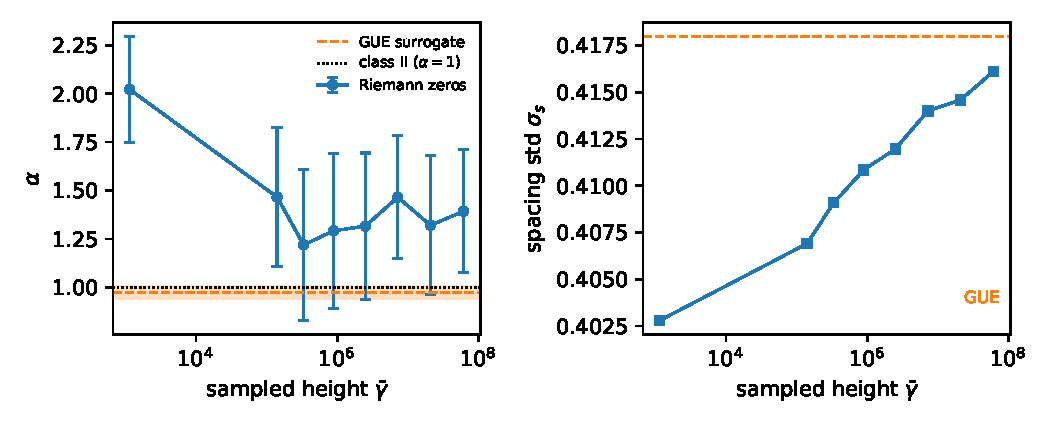
\includegraphics[width=\columnwidth]{../figures/fig3_alpha_vs_height.pdf}
\caption{晶格映射黎曼零点序列的有限高度统计，取自八个互不重叠的窗口，每窗口 $24\times5352$ 个零点。左：超均匀性指数 $\alpha$ 对采样高度 $\bar\gamma$，图中给出 GUE 代理（虚线与阴影带）与 Class~II 值 $\alpha=1$（点线）作参照。加权平均为 $\alpha=1.49\pm0.12$，但 $\alpha$ 无高度依赖：拟合斜率为 $-0.138\pm0.075$（$1.8\sigma$），且完全由最低窗口承担，上方七点平坦（$+0.013\pm0.149$，对 $\alpha=1.364\pm0.135$ 的 $\chi^{2}/\mathrm{dof}=0.07$）。右：同批窗口上的最近邻间距弥散 $\sigma_s$，八个点全部单调上升，外推于 $\bar\gamma\sim10^{8.4}$ 附近达到 GUE 值。短程刚性随高度漂移，而 $k\to0$ 指数不漂移。}
\label{fig:height}
\end{figure}

第二项系统效应值得注意。以随机翻转一部分格点的方式强制目标组分，会在 $s(k)$ 上叠加一个相对大小为 $\sim f/[c(1-c)]$ 的白分量；在 Class~I 序列上 $f\sim10^{-3}$ 即足以测出 $\alpha\approx0$。因此每个生成器都必须\emph{按构造}达到目标组分。

物理含义仍然是有利的：$\alpha\simeq1.4$ 将式~\eqref{eq:master} 的压制从 $\omega^{5}$ 加深到约 $\omega^{5.4}$。凡需要干净的 $\alpha=1$ 参照处，我们使用 GUE 代理，其在同一分析下给出 $\alpha=0.973\pm0.029$。

\subsection{输运观测量}

对每个横向波矢 $k_\parallel^{(m)}$ 构造一条有效一维链，完整保留层间与更远近邻力常数而不作截断。使用三条互为冗余的路径：(i) 由带周期性重正交化的转移矩阵乘积给出的最小 Lyapunov 指数 $\gamma(\omega)$，成本 $\mathcal{O}(N)$，是获取式~\eqref{eq:master} 指数最干净的途径；(ii) 由递归格林函数求值的 Landauer 透射 $\Tr(\omega)=\sum_m\Tr_m(\omega)$；(iii) 用于 $D(\omega)$ 的核多项式方法，它同时验证 Class~II 序列\emph{不}产生谱隙——这是一个必须明确报告的负结果，因为能隙的形成需要 GUE 类序列所不具备的 Bragg 峰。下文每一步的实现，包括用于式~\eqref{eq:unfold} 的 Riemann--Siegel 零点搜索与图~\ref{fig:height} 所施加的窗口不相交约束，均见随附仓库。

\section{观测量提案与设计指标}
\label{sec:observable}

\subsection{为何必须做差分}

低温下总弛豫率按 Matthiessen 规则分解，
\begin{equation}
  \frac{1}{\tau_{\rm tot}}
    = \underbrace{\frac{v}{L_{\rm eff}}}_{\rm Casimir}
    + \frac{1}{\tau_{\rm anh}(\omega,T)}
    + \frac{1}{\tau_{\rm def}(\omega)}
    + \frac{1}{\tau_{\rm iso}(\omega;s)} .
  \label{eq:matthiessen}
\end{equation}
只有最后一项依赖同位素\emph{排布}。Casimir 边界项~[17,18]与频率无关，且在整个亚太赫兹波段超过同位素项，因此任何绝对测量都被背景主导。

考虑两块样品，分别承载 Class~II 与随机排布，且具有相同的同位素组分、几何尺寸、表面工艺、生长批次与点缺陷密度。此时二者的哈密顿量仅相差一个质量置换；式~\eqref{eq:matthiessen} 前三项逐项相同，于是
\begin{equation}
  \Delta\!\left(\frac{1}{\tau}\right)
    = \frac{1}{\tau_{\rm iso}^{\rm rand}(\omega)}\big[1-\mathcal{R}(\omega)\big].
  \label{eq:diffrate}
\end{equation}

组分匹配这一条是承重的。失配 $\delta c$ 会在 $g_2$ 中产生伪差异；在 $c=0.5$ 附近首阶抵消，但二阶项在 $\delta c\sim1\%$ 时仍可达到目标效应的量级。组分必须匹配至 $\delta c<0.2\%$，由二次离子质谱验证，并独立地由拉曼 $E_{2g}$ 峰位标定——该峰位从 h-\tenB N 的 $1394$~cm$^{-1}$ 移至 h-\elevenB N 的 $1358$~cm$^{-1}$~[19]。

透射并非弛豫率的线性函数。取 $\Tr_m=(1+L/\Lambda_m)^{-1}$、$\Lambda_m=v_m\tau_m$，
\begin{equation}
  \Delta\Tr(\omega)\simeq\sum_m \Tr_m^{2}\,\frac{L}{v_m}\,
    \frac{1}{\tau_{{\rm iso},m}^{\rm rand}}\big[1-\mathcal{R}(\omega)\big].
  \label{eq:dT}
\end{equation}
背景从信号中抵消，但不从灵敏度中抵消：前因子 $\Tr_m^{2}$ 保留了全部背景散射，因此样品必须保持准弹道，$L\lesssim\Lambda_{\rm background}$。

\subsection{横向积分不破坏标度律}

一个自然的反对意见是，三维样品中对 $k_\parallel$ 的积分会抹平一维序列效应。对准周期超晶格中的 Cantor 型能隙，该反对成立：能隙位置逐通道迁移，求和后被抹为连续谱。对幂律标度则不成立。式~\eqref{eq:angavg} 的角平均\emph{正是}连续极限下的通道求和；其效果是原样保留指数 $\omega^{4+\alpha}$，仅改变前因子 $2/(\alpha+2)$。指数是标度不变量，对通道平均免疫。

这正是我们采用三维厚样品几何而非纳米带的原因。对本观测量而言量子化 $k_\parallel$ 并无必要，而为此引入的边缘会带来按 $\Delta^{2}\omega^{2}/vW$ 标度的漫散射（见附录），它在低频端必然主导 $\omega^{4+\alpha}$。

\subsection{液氦温区的可行窗口}
\label{sec:feasibility}

取 h-BN 面内参数 $v\simeq2\times10^{4}$~m\,s$^{-1}$ 与 $V_0=9.05$~\AA$^{3}$/原子。等摩尔 \tenB/\elevenB\ 硼子晶格有 $g_2^{\rm B}=2.245\times10^{-3}$，但只有声子本征矢的硼投影有贡献：对长波声学模 $|\bm e(\kappa)|^{2}=M_\kappa/\sum_{\kappa'}M_{\kappa'}$，给出硼权重 $10.81/(10.81+14.01)=0.436$，故有效 $g_2=0.436\times2.245\times10^{-3}=9.8\times10^{-4}\simeq1\times10^{-3}$。据此
\begin{equation}
  \frac{1}{\tau_{\rm iso}^{\rm rand}} \simeq 9.0\times10^{-47}\,\omega^{4}\ \ [\text{s}^{-1}].
  \label{eq:isorate}
\end{equation}
在 $T\lesssim4$~K 以下，Umklapp 过程按 $\exp(-\Theta_D/bT)$ 冻结（h-BN 声学支 $\Theta_D\gtrsim400$~K），且正规过程不弛豫动量，故式~\eqref{eq:matthiessen} 中的非谐项可忽略，背景受 Casimir 限制，$1/\tau_B=v/L$。

对设计点 $\ell=1.25$~nm（$f_0=v/2\ell=8$~THz）与 $L=300\,\mu$m（$1/\tau_B=6.7\times10^{7}$~s$^{-1}$）：

\begin{table}[h]
\centering\small
\caption{$T\lesssim4$~K、$\ell=1.25$~nm、$L=300\,\mu$m 时差分观测量的可行性。}
\label{tab:window}
\begin{tabular}{ccccc}
\hline\hline
$f$ (THz) & $\tau_{\rm iso}^{-1}$ (s$^{-1}$) & $\tau_B/\tau_{\rm iso}$ &
$\mathcal{R}$ & $\Delta\tau_{\rm tot}^{-1}/\tau_{\rm tot}^{-1}$ \\
\hline
4 & $3.6\times10^{7}$ & 0.53 & 0.50 & 17\% \\
5 & $8.8\times10^{7}$ & 1.3  & 0.63 & 21\% \\
6 & $1.8\times10^{8}$ & 2.7  & 0.75 & 18\% \\
7 & $3.4\times10^{8}$ & 5.0  & 0.88 & 10\% \\
8 & $5.8\times10^{8}$ & 8.6  & 1.00 & 0    \\
\hline\hline
\end{tabular}
\end{table}

可及窗口为 $4$--$7$~THz，最优点在 $5$--$6$~THz 附近，预期差分信号 $\Delta\Tr/\Tr\sim20\%$。两个边界互相挤压：下边界由 Casimir 背景设定，压低它需要更大的 $L$，但受准弹道条件封顶；上边界为 $f_0=v/2\ell$，抬高它需要更小的 $\ell$，但下受式~\eqref{eq:designrule} 以及 GUE 间距分布在离散晶格上的可分辨性所限。两条约束交于 $\ell\simeq1.25$~nm，我们以此作为设计指标。

以上数值假定面内传播与面内调制。沿堆垛轴调制对逐层生长更易实现，但其 $v_c\simeq3.5\times10^{3}$~m\,s$^{-1}$ 会把 $f_0$ 下移约六倍，从而关闭与 Casimir 交叉点的重叠区。

\subsection{制备指标及其现状}

上述窗口要求在 $300\,\mu$m 尺度上实现 $1.25$~nm 间距的同位素放置，即约 $2.4\times10^{5}$ 个独立指定的调制单元。我们明确声明：目前没有任何 h-BN 生长技术达到该指标。沿 $c$ 轴的 MOCVD 前驱体切换提供层级控制，但相干调制长度约为 $1\,\mu$m；面内纳米分辨的同位素图案化尚无成熟路径。

因此本文定位为理论与设计指标研究。其贡献是式~\eqref{eq:master} 的标度律、隐形窗口定理、式~\eqref{eq:designrule} 的离散化界，以及对观测窗口及达成它所需生长能力的定量界定。我们认为明确陈述这一差距比掩盖它更有用。

\section{结论}

在固定同位素方差下，同位素的空间排布是一个真实且此前未被使用的声子输运控制参数。通过质量涨落结构因子推广 Tamura 理论，得到 $\tau_{\rm iso}^{-1}\propto\omega^{\,d+1+\alpha}$，其中超均匀性指数以可加且与维度无关的方式贡献。将 GUE 类序列映射到 \tenB/\elevenB\ 调制上，把瑞利的 $\omega^{4}$ 转换为 $\omega^{5}$；由有限高度黎曼零点构成的序列更为刚性，给出与所采样高度无关的 $\alpha=1.49\pm0.12$ 及相应更深的压制。对隐形排布，我们证明黄金规则速率在 $vK/2$ 以下恒等于零，从而定义了一个硬边界的透明窗口。

六方氮化硼是天然的载体：其硼子晶格带有反常巨大的天然质量无序（$g_2\approx1.35\times10^{-3}$，约为天然碳的十八倍），而氮子晶格几乎同位素纯，且其力常数在替换下严格不变。

\medskip\noindent
\emph{数据可用性.} 全部代码、生成的序列与稿件源码公开于 \url{https://github.com/Ruqing1963/hbn-hyperuniform-isotope}。该仓库从一次原胞力常数计算出发复现全部图件以及第~\ref{sec:methods}~与~\ref{sec:observable}~节所引的每一个数值，并包含针对式~\eqref{eq:master} 标度指数的回归测试。


\section*{附录：边界粗糙度标度}
\setcounter{equation}{0}
\renewcommand{\theequation}{A\arabic{equation}}

以 Ziman 镜面参数 $p(\omega)=\exp(-4q^{2}\Delta^{2})$ 描述均方根粗糙度 $\Delta$，漫射边界速率为
\begin{equation}
  \frac{1}{\tau_{\rm edge}}=\big[1-p(\omega)\big]\frac{v}{W}
  \;\xrightarrow{\;q\Delta\ll1\;}\;
  \frac{4\Delta^{2}}{vW}\,\omega^{2}.
  \label{eq:edge}
\end{equation}
与式~\eqref{eq:master} 比较可见，只要 $d+1+\alpha>2$（即恒成立），边界散射就在低频端占主导。令二者相等给出交叉宽度
\begin{equation}
  W_{\rm cross}=\frac{16\pi\Delta^{2}v^{2}}{V_0\,g_2\,\omega^{2}},
  \label{eq:wcross}
\end{equation}
对 $\Delta=0.5$~nm、$f=1$~THz 其量级为 $10^{2}\,\mu$m。任何窄到足以量子化 $k_\parallel$ 的几何都会被边界散射主导四到六个数量级，这从定量上排除了纳米带路线。

\section*{参考文献}
{\footnotesize
\begin{enumerate}\itemsep0pt
\item K.~Chen \textit{et al.}, Ultrahigh thermal conductivity in isotope-enriched cubic boron nitride, \textit{Science} \textbf{367}, 555--559 (2020).
\item C.~Yuan \textit{et al.}, Modulating the thermal conductivity in hexagonal boron nitride via controlled boron isotope concentration, \textit{Commun. Phys.} \textbf{2}, 43 (2019).
\item A.~J.~Giles \textit{et al.}, Ultralow-loss polaritons in isotopically pure boron nitride, \textit{Nat. Mater.} \textbf{17}, 134--139 (2018).
\item S.~Tamura, Isotope scattering of dispersive phonons in Ge, \textit{Phys. Rev. B} \textbf{27}, 858--866 (1983).
\item P.~G.~Klemens, The scattering of low-frequency lattice waves by static imperfections, \textit{Proc. Phys. Soc. A} \textbf{68}, 1113--1128 (1955).
\item S.~Torquato, Hyperuniform states of matter, \textit{Phys. Rep.} \textbf{745}, 1--95 (2018).
\item S.~Torquato and F.~H.~Stillinger, Local density fluctuations, hyperuniformity, and order metrics, \textit{Phys. Rev. E} \textbf{68}, 041113 (2003).
\item C.~E.~Zachary and S.~Torquato, Hyperuniformity in point patterns and two-phase random heterogeneous media, \textit{J. Stat. Mech.} P12015 (2009).
\item S.~Torquato, A.~Scardicchio and C.~E.~Zachary, Point processes in arbitrary dimension from fermionic gases, random matrix theory, and number theory, \textit{J. Stat. Mech.} P11019 (2008).
\item H.~L.~Montgomery, The pair correlation of zeros of the zeta function, in \textit{Analytic Number Theory}, Proc. Sympos. Pure Math. \textbf{24} (AMS, 1973), pp. 181--193.
\item A.~M.~Odlyzko, On the distribution of spacings between zeros of the zeta function, \textit{Math. Comp.} \textbf{48}, 273--308 (1987).
\item N.~H.~Protik and C.~Draxl, Beyond the Tamura model of phonon-isotope scattering, \textit{Phys. Rev. B} \textbf{109}, 165201 (2024).
\item R.~D.~Batten, F.~H.~Stillinger and S.~Torquato, Classical disordered ground states, \textit{J. Appl. Phys.} \textbf{104}, 033504 (2008).
\item H.~M.~Edwards, \textit{Riemann's Zeta Function} (Academic Press, New York, 1974).
\item I.~Dumitriu and A.~Edelman, Matrix models for beta ensembles, \textit{J. Math. Phys.} \textbf{43}, 5830--5847 (2002).
\item M.~V.~Berry, Semiclassical formula for the number variance of the Riemann zeros, \textit{Nonlinearity} \textbf{1}, 399--407 (1988).
\item H.~B.~G.~Casimir, Note on the conduction of heat in crystals, \textit{Physica} \textbf{5}, 495--500 (1938).
\item J.~M.~Ziman, \textit{Electrons and Phonons} (Oxford University Press, Oxford, 1960).
\item T.~Q.~P.~Vuong \textit{et al.}, Isotope engineering of van der Waals interactions in hexagonal boron nitride, \textit{Nat. Mater.} \textbf{17}, 152--158 (2018).
\end{enumerate}}

\end{document}
